% !TeX spellcheck = cs_CZ
%{\tikzset{external/prefix={tikz/FYZII/}}
% \tikzset{external/figure name/.add={ch01_}{}}
%---------------------------------------------------------------------------------------------------
% file fey1ch01_02_03.tex
%---------------------------------------------------------------------------------------------------
%================ Kapitola: Elektromagnetizmus======================================================
\chapter{Elektromagnetizmus}\label{fyz:IIchapI}
\minitoc

  %-------------- Elektrické síly ------------------------------------------------------------------
  \section{Elektrické síly}
    \cite[s.~13]{Feynman02} Představme si sílu, která se podobá gravitaci a mění se převážně nepřímo
    úměrně druhé mocnině vzdálenosti, ale asi miliardu miliard miliard miliard-krát větší. A ještě 
    s jedním rozdílem. Nechť existují dva druhy „látky“, nazývejme je kladná a záporná. Nechť na 
    rozdíl od gravitace, v níž existuje pouze přitahování, se stejné druhy odpuzují a odlišné druhy 
    přitahují. Co by se stalo?
    
    Chomáč kladné látky by se ohromnou silou odpuzoval a rozptýlil by se na všechny strany. S 
    chomáčem záporné by se stalo totéž. Ale směs stejného množství kladné a záporné látky by se 
    chovala zcela odlišně. Ohromná přitažlivá síla by přitáhla opačné kousky k sobě. V konečném 
    důsledku by se tyto úžasné síly navzájem téměř dokonale vykompenzovaly vytvořením hutných 
    jemných směsí kladného a záporného, přičemž mezi dvěma oddělenými chomáči takových směsí by 
    neexistovalo téměř žádné přitahování nebo odpuzování.
    
    \begin{wrapfigure}[19]{r}{5cm}
      \centering
      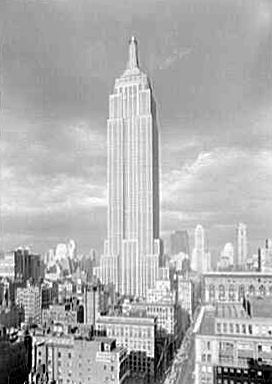
\includegraphics[width=0.9\linewidth]{fyz_fig145.jpg}
      \caption{Empire State Building, 1934}
      \label{fyz:fig145} 
    \end{wrapfigure} 
    Taková síla existuje - je to \emph{elektrická síla}! A každá látka je směsí kladných protonů a 
    záporných elektronů, které se touto velkou silou přitahují a odpuzují. Ale vyvážení je tak 
    dokonalé, že když stojíte blízko někoho jiného, necítíte sílu vůbec žádnou. Kdyby existoval jen 
    malý zbytek nerovnováhy, poznali bychom to. Kdybyste stáli od někoho na vzdálenost paže a každý 
    z vás by měl o jedno procento víc elektronů než protonů, byla by odpudivá síla mezi vámi 
    neuvěřitelná. Jak velká? Dost na to, aby zvedla obrovský mrakodrap? Ne! Aby zvedla Mount 
    Everest? Ne! Odpuzování by stačilo na zvednutí břemene s hmotností celé zeměkoule!

    S ohledem na tak perfektní vyvážení ohromné síly, působící v této směsi, není těžké pochopit, 
    že látka s tendencí udržet své kladné a záporné náboje v nejjemnější rovnováze může 
    mít velkou tvrdost a pevnost. Mrakodrap \wikiELB se například vychyluje ve větru jen o necelé 
    tři metry, neboť elektrické síly udržují každý elektron a proton víceméně ve stálé poloze. Na 
    druhé straně, když se podíváme na tak malé množství látky, že uvidíme jen několik atomů, 
    libovolná malá část látky obvykle nebude mít stejný počet kladných a záporných; nábojů, 
    takže budou existovat velké zbytkové elektrické síly. I kdyby byly počty obou druhů nábojů ve 
    dvou sousedních malých částech stejné, pravděpodobně ještě zůstanou mezi oběma částmi 
    elektrické síly, neboť síly mezi jednotlivými náboji se mění nepřímo úměrně s druhou mocninou 
    vzdálenosti. Zbytková síla může vzniknout, nachází-li se záporný náboj jedné části blíž 
    kladnému náboji než kladný náboj zápornému v části jiné. Pak mohou být přitažlivé síly větší 
    než odpudivé a může dojít k výslednému přitahování i dvou částí bez nadbytečných nábojů. Síla, 
    která “udržuje” pohromadě atomy, a chemická síla, která drží molekuly, jsou ve skutečnosti 
    elektrickými silami působícími v oblastech s nedokonalou rovnováhou nábojů anebo s velmi malými 
    vzdálenostmi.

    Samozřejmě víme, že se atomy skládají z kladných protonů v jádře a záporných elektronů v jeho 
    okolí. Můžeme se ptát: Když je tato elektrická síla tak úžasná, proč spolu protony a elektrony 
    nesplynou? Když mají tvořit dokonalou směs, proč tato směs není ještě dokonalejší? Odpověď 
    nacházíme v kvantových jevech. Pokusíme-li se naše elektrony uzavřít do oblasti těsně 
    přiléhající k protonům, musí mít podle principu neurčitosti nenulovou střední kvadratickou 
    hybnost, která je tím větší, čím těsnější je ohraničení. Právě tento pohyb, vyplývající ze 
    zákonů kvantové mechaniky, zabraňuje elektrické přitažlivosti dostat náboje jakýmkoli způsobem 
    blíž k sobě.
    
    Je tu další otázka: Co drží pohromadě atomové jádro? V jádře je několik kladných protonů. Proč 
    se od sebe neoddělí? Ukazuje se, že v jádře existují kromě elektrických i neelektrické síly, 
    které se nazývají jaderné síly. Jsou větší než elektrické síly a jsou schopné držet protony u 
    sebe i přes jejich elektrické odpuzování. Síly jádra však mají malý dosah - jejich velikost 
    klesá mnohem rychleji než \(\frac{1}{r^2}\). A to má důležitý důsledek. Kdyby jádro obsahovalo 
    velmi mnoho protonů, stalo by se příliš velkým a nezůstalo by pohromadě. Příkladem je uran s 
    \(92\) protony. Jaderné síly působí převážně jen mezi každým protonem (nebo neutronem) a jeho 
    nejbližším sousedem, ale elektrické síly působí i na větší vzdálenosti a vyvolávají tak 
    odpuzování každého protonu od všech ostatních v jádře. Čím víc je v jádře protonů, tím je 
    elektrické odpuzování silnější, až dokud - jako v případě uranu - není rovnováha tak křehká, že 
    je jádro účinkem elektrické síly téměř připraveno se rozletět. Jestliže takové jádro jen trochu 
    „postrčíme“ (pokud do něj vyšleme pomalý neutron), rozdělí se na dvě části s kladným nábojem. V 
    důsledku elektrického odpuzování od sebe obě části odletí. Energie, která se při tom 
    uvolňuje, je energií atomové bomby. Obvykle se tato energie nazývá jaderná, ale v podstatě je 
    to elektrická energie uvolněná tehdy, když elektrické síly překonaly přitažlivé síly jádra.
    
    Konečně se můžeme ptát, co drží pohromadě záporný elektron (neboť ten nemá žádné jaderné síly). 
    Skládá-li se elektron celý z jednoho druhu látky, každá z jeho částí by měla odpuzovat ty 
    ostatní. Proč se tedy nerozletí? Má však elektron „části“? Asi bychom měli říct, že elektron je 
    jen bod a že elektrické síly působí jen mezi různými dvěma bodovými náboji, takže sám na sebe 
    elektron nepůsobí. Snad. Vše, co můžeme říct, je, že otázka, co drží pohromadě elektron, 
    způsobila v pokusech o vytvoření úplné teorie elektromagnetizmu mnoho těžkostí. Tato otázka 
    zatím nebyla zodpovězena. V dalších kapitolách se budeme tomuto tématu věnovat více.
    
    Jak jsme viděli, je třeba čekat, že právě kombinace elektrických sil a kvantově mechanických 
    jevů bude určovat detailní strukturu makroskopických množství látek, a tím i jejich vlastnosti. 
    Některé látky jsou tvrdé, jiné měkké. Některé jsou elektrickými vodiči, protože jejich 
    elektrony se mohou volně pohybovat, jiné jsou izolátory, protože jejich elektrony jsou pevné 
    připoutané k jednotlivým atomům. Později budeme hovořit o tom, jak vznikají některé z těchto 
    vlastností. Je to však složitá otázka, proto nejdřív budeme zkoumat elektrické síly jen v 
    jednoduchých situacích. Začněme s probíráním zákonů elektřiny, včetně magnetizmu, který je 
    vlastně částí téhož předmětu.

    O přítomnosti elektrického náboje se tedy přesvědčujeme pouze na základě jeho silového projevu.
    Znamená to, že existenci jednoho jediného náboje bychom nemohli nijak odhalit. Kdyby
    existovaly pouze dva náboje, mohli bychom určit, zda jsou souhlasného či nesouhlasného
    znamení, nemohli bychom však rozhodnout ani o znamení, ani o velikosti těchto nábojů. Teprve
    jsou-li k dispozici alespoň tři náboje, můžeme jeden z nich vybrat jako jednotkový a kladný a
    ze silového působení určit velikost a znamení druhých nábojů. Tato síla podobně jako gravitační 
    klesá nepřímo úměrně s druhou mocninou vzdálenosti mezi náboji. Tento vztah se nazývá 
    \hyperlink{fyz:IIchapIVsecII}{Coulombův zákon}. Ale neplatí přesně, když se náboje pohybují, 
    protože elektrické síly závisí také na pohybu nábojů, a to komplikovaným způsobem. Jednu část 
    síly mezi pohybujícími se náboji nazýváme \emph{magnetická síla}, která vlastně představuje 
    jeden aspekt elektrického účinku. Právě proto hovoříme o „elektromagnetizmu“.
    
    Existuje důležitý obecný princip, který umožňuje zacházet s elektromagnetickými silami poměrně 
    snadno. Experimentálně se zjistilo, že síla působící na náboj závisí pouze na poloze tohoto 
    náboje, jeho rychlosti a velikosti, bez ohledu na to, kolik dalších nábojů existuje a jak se 
    pohybují. Sílu \(\vec{F}\) působící na náboj \(q\), který se pohybuje rychlostí \(\vec{v}\), 
    můžeme vyjádřit takto:
    \begin{equation}\label{FYZ:eq_fey_elmag01}
      \boxed{\vec{F} = q(\vec{E}+\vec{v}\times\vec{B})}\, ,
    \end{equation}
    kde \(\vec{E}\) je \emph{elektrické pole} a \(\vec{B}\) \emph{magnetické pole} v místě, kde se 
    nachází náboj. Důležité je, že elektrické síly všech nábojů ve vesmíru lze složit právě z 
    těchto dvou vektorů. Jejich hodnoty závisí na tom, kde se uvažovaný náboj nachází, a mohou se v 
    čase měnit. Kromě toho, nahradíme-li tento náboj jiným, změní se síla působící na nový náboj v 
    poměru velikostí obou nábojů, nezmění-li všechny ostatní náboje na světě svou polohu nebo 
    pohyb. (Samozřejmě že v reálné situaci každý náboj působí na všechny ostatní ve svém okolí a 
    může je uvést do pohybu. A tak když v některých případech nahradíme náš určitý náboj jiným 
    nábojem, mohou se pole změnit.)
    
    Z \ref{part:FYZI}. dílu víme, jak se určuje pohyb částice, známe-li sílu, která na ni působí. 
    Dosadíme-li výraz (\ref{FYZ:eq_fey_elmag01}) do pohybové rovnice, dostaneme
    \begin{equation}\label{FYZ:eq_fey_elmag02}
      \der{ }{t}\left(\frac{m\vec{v}}{\sqrt{1-\frac{v^2}{c^2}}}\right) = \vec{F} =
      q(\vec{E}+\vec{v}\times\vec{B})
    \end{equation}
    Známe-li \(\vec{E}\) a \(\vec{B}\), můžeme určit pohyby nabitých částic. K tomu už jen 
    potřebujeme vědět, jak \(\vec{E}\) a \(\vec{B}\) vznikají.
    
    Jeden z nejdůležitějších zjednodušujících principů vytváření elektrických polí závisí na tomto:
    Předpokládejme, že určitý počet nábojů pohybujících se libovolným způsobem vytvoří pole 
    \(\vec{E_1}\) a jiná množina nábojů vytvoří pole \(\vec{E_2}\). Působí-li obě množiny nábojů 
    současně (při zachování stejných pohybů a poloh, které měly, když jsme o nich uvažovali 
    odděleně), vytvoří pole, které je dáno součtem
    \begin{equation}\label{FYZ:eq_fey_elmag03}
      \vec{E} = \vec{E_1} + \vec{E_2}
    \end{equation}
    Tento fakt se nazývá princip \emph{superpozice polí}. Platí také pro magnetická pole.
    
    Z tohoto principu vyplývá, že budeme-li vědět, podle jakého zákona vytváří elektrická a 
    magnetická pole jediný náboj pohybující se libovolným způsobem, zákony elektrodynamiky už budou 
    úplné. Chceme-li znát sílu působící na náboj \(A\), je třeba spočítat pouze \(\vec{E}\) a 
    \(\vec{B}\), které vytváří každý náboj \(B\), \(C\), \(D\) atd., pak vypočítat vektory 
    \(\vec{E}\) a \(\vec{B}\) všech nábojů, a tak najít  pole a síly působící z nich na \(A\). 
    Kdyby se ukázalo, že zákon, podle kterého se vytváří pole jediného náboje, je jednoduchý, byla 
    by to nejšikovnější cesta, jak popsat zákony elektrodynamiky. My už jsme uvedli tento zákon 
    (kapitola \ref{fyz:IchapXXVIII}, díl \ref{part:FYZI}), který je, bohužel, dost složitý.
    
    Ukazuje se, že tvar, ve kterém jsou zákony elektrodynamiky nejednodušší, není tím tvarem, který 
    bychom zde mohli očekávat. Není totiž vůbec jednoduché udat vzorec síly, kterou působí jeden 
    náboj na druhý. Je pravda, že pokud jsou náboje v klidu, je výraz pro Coulombovu sílu ještě 
    jednoduchý, ale když se náboje pohybují, vztahy se komplikují kromě jiného i časovým zpožděním 
    a zrychlením. Z tohoto důvodu nehodláme prezentovat elektrodynamiku pouze prostřednictvím 
    zákonů síly působící mezi náboji; pokládáme za vhodnější jiné hledisko - při něm jsou zákony 
    elektrodynamiky zvládnutelné snáze.
    
    \begin{note}
      Co je vlastní podstatou elektrického náboje nevíme. Na základě poznatků současné mikrofyziky 
      (rok 2000) jej můžeme považovat za jednu z vlastností elementárních částic, která podmiňuje 
      jejich vzájemné působení. Rozlišujeme čtyři základní typy vzájemného působení 
      (\emph{interakce}) mezi elementárními částicemi: \emph{gravitační, slané elektromagnetické a 
      silné}. Gravitační interakce je univerzální a týká se všech částic. Setkali jsme se s ní v 
      mechanice, její velikost udává Newtonův gravitační zákon a její podstatu se snaží objasnit 
      obecná teorie relativity. Slabá interakce se projevuje u některých typů radioaktivního 
      rozpadu za účasti neutrina. Podobně elektromagnetická interakce se uplatňuje mezi 
      elementárními částicemi a jednou z jejích charakteristik je náboj. Silná interakce existuje 
      mezi částicemi, které nazýváme hadrony, a drží pohromadě atomové jádro, které by se jinak 
      odpudivými elektrickými silami působícími mezi protony musely rozdělit.
      
      Současný rozvoj mikrofyziky naznačuje, že hadrony, které jsme dříve považovali za
      elementární, mají svoji strukturu a komponenty. Předpokládáme o nich, že jsou tvořeny tzv.
      kvarky. Na současné úrovni vystupují tedy jako elementární kvarky a leptony (k nim patří
      elektron, mion, tauon a odpovídající neutrina), jejich antičástice a dále pak částice, které
      zprostředkovávají interakci mezi nimi.
    \end{note}
    
    %------------- Elektrická a magnetická pole ----------------------------------------------------
    \section{Elektrická a magnetická pole}
      Nejdříve si musíme trochu rozšířit naši představu o elektrickém vektoru \(\vec{E}\) a 
      magnetickém vektoru \(\vec{B}\). Definovali jsme je pomocí sil působících na náboj. Nyní 
      chceme hovořit o elektrických a magnetických polích v bodě, i v tom případě, kdy se v něm 
      nenachází žádný elektrický náboj. Tvrdíme: jestliže existují síly působící na náboj, existuje 
      tam „něco“ i tehdy, je-li náboj odstraněn. Když na náboj umístěný v bodě \((x, y, z)\) působí 
      v čase \(t\) síla \(\vec{F}\) daná výrazem (\ref{FYZ:eq_fey_elmag01}), přiřazujeme bodu \((x, 
      y, z)\) v prostoru vektory \(\vec{E}\) a \(\vec{B}\). O vektorech \(\vec{E}(x,y, z, t)\) a 
      \(\vec{B}(x, y, z, t)\) si můžeme myslet, že určují síly, které by působily v čase \(t\) na 
      náboj umístěný v bodě \((x, y, z)\) za podmínky, že umístění náboje do bodu \((x, y, z)\) 
      neporuší polohy nebo pohyby žádných jiných nábojů vytvářejících i pole \(\vec{E}\) a 
      \(\vec{B}\).
    
      Podle této představy připíšeme každému bodu \((x, y, z)\) v prostoru dva vektory \(\vec{E}\) 
      a \(\vec{B}\), které se mohou měnit v čase. Elektrická a magnetická pole pak chápeme jako 
      \emph{vektorové funkce} proměnných \(x\), \(y\), \(z\) a \(t\). Protože vektor je určen svými 
      složkami, každé z polí \(\vec{E}(x, y, z, t)\) a \(\vec{B}(x, y, z, t)\) představuje tři 
      reálné funkce proměnných \(x\), \(y\), \(z\) a \(t\).
      
      \begin{figure}[ht!]
        \centering
        \begin{tabular}{cc}
          \subfloat[ ]{\label{fyz:fig146a}
            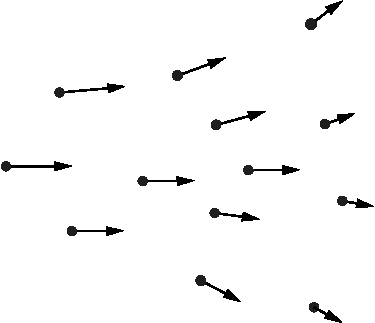
\includegraphics[width=0.35\linewidth]{fyz_fig146a.pdf}
          }                                                               &
          \hspace{0.1\linewidth}
          \subfloat[]{\label{fyz:fig146b}
            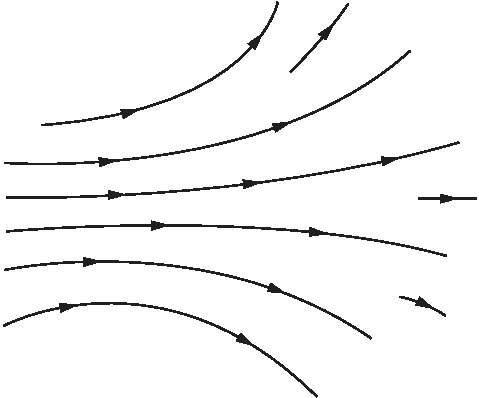
\includegraphics[width=0.35\linewidth]{fyz_fig146b.pdf}
          }  
        \end{tabular}
        \caption{Znázornění vektorového pole: a) šipkami, jejichž velikosti a směry  udávají 
                 hodnoty vektorového pole v bodech, ze kterých vycházejí; b) siločar, jejichž tečny 
                 mají v každém bodě směr vektoru pole a jejichž hustota je úměrná velikostí vektoru 
                 pole \cite[s.~17]{Feynman02}}
        \label{fyz:fig146}
      \end{figure} 
      Právě proto, že \(\vec{E}\) (nebo \(\vec{B}\)) je možné určit v každém bodě v prostoru, 
      nazývá se pole. Pole je jakákoliv fyzikální veličina, která nabývá různé hodnoty v různých 
      bodech prostoru. Například teplota je polem - v tomto případě skalárním polem, které 
      zapisujeme jako \(T(x, y, z)\). Teplota se může také měnit v čase, říkáme, že je závislá na 
      čase a zapisujeme ji jako \(T(x, y, z, t)\). Jiným příkladem  je „rychlostní pole“ tekoucí 
      kapaliny. Rychlost kapaliny v každém bodě prostoru v čase \(t\) zapisujeme jako \(\vec{v}(x, 
      y, z, t)\). Je to vektorové pole.
    
      Vraťme se k elektromagnetickým polím. Ačkoliv se jejich závislost na nábojích, které je 
      vytvořily, vyjadřuje složitými vzorci, mají důležitou následující vlastnost: vztahy mezi 
      hodnotami polí v \emph{jednom bodě} a hodnotami polí v \emph{bodech sousedních} jsou velice 
      jednoduché. Pole lze zcela popsat pomocí několika vztahů, které mají tvar diferenciálních 
      rovnic. Právě pomocí takových rovnic se zapisují zákony elektrodynamiky nejjednodušeji.
    
      Existují rozmanité nápady, jak si vytvořit představu o chování polí. Nejsprávnější z nich je i
      nejabstraktnější: pole chápeme prostě jako matematické funkce polohy a času. Můžeme se 
      pokusit získat představu pole také tím, že si v mnoha bodech prostoru nakreslíme vektory, z 
      nichž každý bude udávat intenzitu a směr pole v daném bodě. Takové zobrazení pole vidíme na 
      obr. \ref{fyz:fig146a}. Můžeme však jít dál a nakreslit křivky, které mají všude vektory 
      ve směru tečny, tj. jakoby šly za šipkami a sledovaly směr pole. Když postupujeme takto, 
      ztrácíme znázornění délek vektory. Intenzitu pole můžeme však znázornit tak, že křivky 
      vykreslíme daleko od sebe, když je pole slabé, a blízko sebe, když je silné. Domluvíme se 
      přitom, že počet křivek připadající na jednotku plochy postavenou kolmo na křivky 
      bude přímo úměrný intenzitě pole. Toto je ovšem jen zjednodušení a vyžaduje, aby se tu a tam 
      objevily nové křivky tak, aby jejich počet vždy souhlasil s intenzitou pole. Pole z obr. 
      \ref{fyz:fig146a} je znázorněno pomocí těchto siločár na obr.\ref{fyz:fig146b}.

        
  %-------------- Charakteristiky vektorových polí -------------------------------------------------
  \section{Charakteristiky vektorových polí}
    V našem popisu zákonů elektřiny, který se opírá o pojem pole, budeme používat dvě matematicky 
    důležité vlastnosti vektorového pole. Předpokládejme, že máme nějakou uzavřenou plochu, a ptáme 
    se, zda se „něco“ ztrácí z jejího nitra, tj. zda má pole vlastnost „výtoku“. Například případě 
    rychlostního pole bychom se mohli ptát, zda rychlost směřuje vždy ven z plochy, nebo obecněji, 
    zda víc kapaliny (za jednotku času) vytéká než vtéká. Výsledné množství kapaliny, vytékající z 
    určité plochy za jednotku času, se nazývá tok rychlosti plochou. Tok elementární ploškou je 
    roven složce rychlosti kolmé na plošku, násobené velikostí plošky. Pro libovolnou uzavřenou 
    plochu je čistý výtok, nebo krátce tok, roven součinu jejího plošného obsahu a střední 
    normálové složky rychlosti, orientované ven z objemu uzavřeného plochou:    
    \begin{equation}\label{FYZ:eq_fey_elmag04}
      \text{Tok} = (\text{Střední normálová složka}) \cdot (\text{plošný obsah})
    \end{equation}
    
    \begin{figure}[ht!]
      \centering
      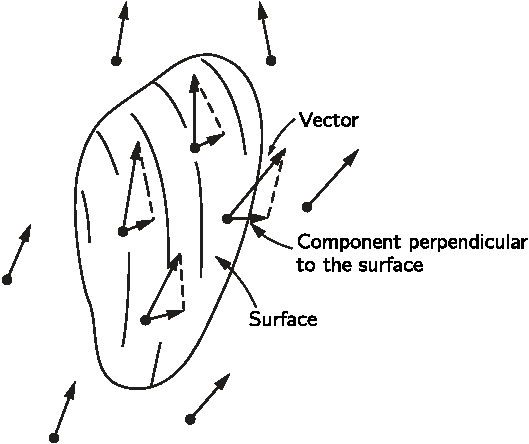
\includegraphics[width=0.7\linewidth]{fyz_fig147.pdf}
      \caption{Tok vektorového pole plochou se definuje jako součin střední hodnoty normálové 
               složky vektoru a obsahu plochy. \cite[s.~18]{Feynman02}}
      \label{fyz:fig147} 
    \end{figure}
     
    I v případě elektrického pole můžeme matematicky definovat veličinu analogickou k toku. Opět ji 
    nazveme tokem, ale samozřejmě nepůjde o tok nějaké látky, protože elektrické pole není 
    rychlostí něčeho. Ukazuje se však, že i tak je matematická veličina udávající střední 
    normálovou složku pole velice užitečná. Pak hovoříme o elektrickém toku, definovaném taktéž 
    podle (\ref{FYZ:eq_fey_elmag04}). Přitom je užitečné zavést tok nejen zcela uzavřenou plochou, 
    ale jakoukoliv ohraničenou plochou. Podobně jako předtím se tok takovouto plochou definuje jako 
    součin jejího plošného obsahu a střední normálové složky vektoru. Tyto pojmy ilustruje obr. 
    \ref{fyz:fig147}. 
    
    Druhá vlastnost vektorového pole se týká spíše křivky než plochy. Opět si představme rychlostní 
    pole, které popisuje tok kapaliny. Mohli bychom si položit tuto zajímavou otázku: Cirkuluje 
    kapalina? Myslíme tím toto: existuje výsledný rotační pohyb kapaliny podél nějaké uzavřené 
    křivky? Představme si, že jsme v jeden okamžik zmrazili všechnu kapalinu s výjimkou vnitřku 
    trubice s konstantním průřezem a tvarem uzavřené křivky, jako na obr. \ref{fyz:fyz_fig041c}. 
    Mimo trubici se kapalina zastaví, ale uvnitř se může udržovat v pohybu, a to v závislosti na 
    hybnosti kapaliny zachycené v trubici, tj. podle toho, zda hybnost kapaliny v jednom směru 
    podél trubice je větší než hybnost v opačném směru.  

    \begin{figure}[ht!]
      \centering
      \begin{tabular}{ccc}
        \subfloat[ ]{\label{fyz:fyz_fig041a}
          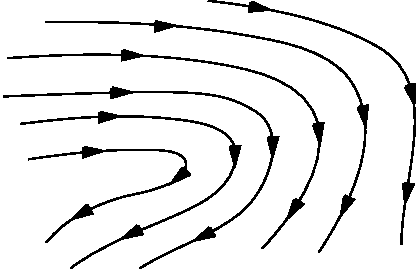
\includegraphics[width=0.25\linewidth]{fyz_fig041a.pdf}
        }                                                                          &
        \subfloat[ ]{\label{fyz:fyz_fig041b}
          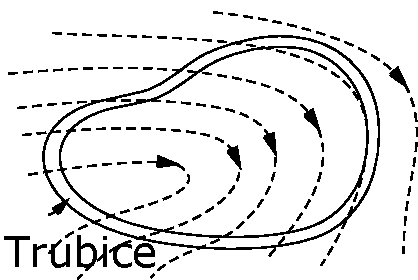
\includegraphics[width=0.28\linewidth]{fyz_fig041b.pdf}
        }                                                                          &
        \subfloat[ ]{\label{fyz:fyz_fig041c}
          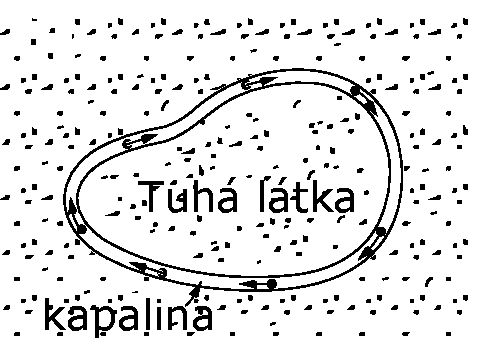
\includegraphics[width=0.30\linewidth]{fyz_fig041c.pdf}
        }
      \end{tabular}
      \caption{Cirkulace vektorového pole: a) Pole rychlosti v kapalině. b) Představme si trubici s
               konstantním průřezem a tvarem nějaké uzavřené křivky. c) Kdyby kapalina všude s
               výjimkou vnitřku trubice náhle zmrzla, v trubici by cirkulovala.
               \cite[s.~18]{Feynman02}}
      \label{fyz:fig041}
    \end{figure}    

    Veličinu nazvanou cirkulace definujeme jako výslednou rychlost kapaliny v trubici násobenou 
    délkou trubice. Naše pojmy můžeme nyní opět rozšířit a cirkulaci definovat pro jakékoliv 
    vektorové pole (i když tam není nic, co by se pohybovalo). Pro libovolné vektorové pole se 
    cirkulace podél libovolné myšlené uzavřené křivky definuje jako střední tangenciální složka 
    vektoru (s ohledem na směr oběhu po křivce) násobená délkou křivky (obr. \ref{fyz:fig042}). 

    \begin{figure}[ht!]  %\ref{fyz:fig042}
      \centering
      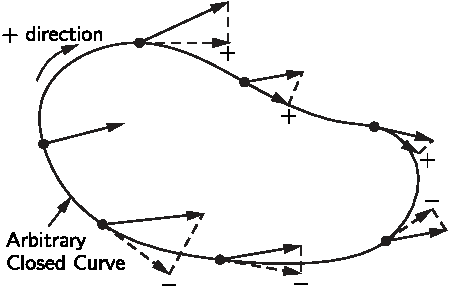
\includegraphics[width=0.7\linewidth]{fyz_fig042.pdf}
      \caption{Cirkulace vektorového pole je rovna součinu střední tangenciální složky 
               vektoru (vzhledem ke směru pohybu po křivce) a délky uzavřené křivky.
               \cite[s.~19]{Feynman02}}
      \label{fyz:fig042}
    \end{figure}
    
    \begin{equation}\label{FYZ:eq_fey_elmag05}
        \renewcommand\arraystretch{0.6} \setlength\minrowclearance{2.4pt}
      \text{Cirkulace} = 
        \left(\begin{array}{c}
          \text{střední}      \\
          \text{tangenciální} \\
          \text{složka}
         \end{array}
       \right)\cdot
       \left(\begin{array}{c}
          \text{délka}      \\
          \text{křivky}
        \end{array}
       \right)
    \end{equation}

    Uvidíme, že z této definice opravdu vyplývá číslo, které je přímo úměrné rychlosti oběhu 
    kapaliny v rychle zamrzlé trubici, popsané předtím.
    
    Právě pomocí těchto dvou pojmů - toku a cirkulace — už můžeme uvést všechny zákony elektřiny a
    magnetizmu. Možná, že význam zákonů hned plně nepochopíme, ale poskytnou nám určitou představu 
    o tom, jak se v konečném tvaru formuluje fyzika elektromagnetických jevů.

  
  %------------- Zákony elektromagnetizmu ----------------------------------------------------------
  \section{Zákony elektromagnetizmu}
    První zákon elektromagnetizmu určuje tok elektrického pole:
    \begin{equation}\label{FYZ:eq_fey_elmag06}
      \text{Tok }\vec{E}_{\substack{\text{ libovolnou}\\\text{uzavřenou}\\\text{křivkou}}}
        = \frac{
          \begin{array}{c}
              \text{celkový náboj}      \\
            \text{uvnitř plochy} 
          \end{array}
       }{\varepsilon_0}
    \end{equation}
    kde \(\varepsilon_0\) je vhodná konstanta (čte se „epsilon nula“). Není-li uvnitř plochy žádný 
    náboj, ačkoliv v jejím okolí náboje jsou, je střední normálová složka \(\vec{E}\) nulová, takže 
    výsledný tok plochou je nulový. Abychom naznačili hloubku tohoto tvrzení, můžeme ukázat, že 
    vztah (\ref{FYZ:eq_fey_elmag06}) je ekvivalentní s Coulombovým zákonem. Stačí doplnit 
    předpoklad, že pole jednotlivého náboje je kulové symetrické. V případě bodového náboje opíšeme 
    kolem náboje kulovou plochu. Střední normálová složka vektoru pole je pak dána právě velikostí 
    \(\vec{E}\) v libovolném bodě kulové plochy, neboť pole má nevyhnutelně radiální směr a v 
    každém bodě na kouli má stejnou intenzitu. Naše pravidlo tvrdí, že součin pole na povrchu koule 
    a plošného obsahu jejího povrchu, tj. tok směrem ven z koule, je přímo úměrný náboji uvnitř 
    koule. Jestliže bychom poloměr koule zvětšili, plošný obsah by vzrostl přímo úměrně druhé 
    mocnině poloměru. Ale střední normálová složka elektrického pole vynásobená zvětšeným plošným 
    obsahem se musí rovnat stejnému náboji uvnitř, a pole se tedy musí zmenšit nepřímo úměrně druhé 
    mocnině poloměru — dostáváme výsledek, že pole je nepřímo úměrné čtverci vzdálenosti.
    
    Vezmeme-li libovolnou pevnou křivku v prostoru a měříme-li podél ní cirkulaci elektrického pole,
    zjistíme, že obecně není rovna nule (i když jde o Coulombovo pole). Pro elektřinu platí totiž i 
    druhý zákon, podle něhož pro jakoukoliv plochu \(S\) (neuzavřenou) ohraničenou křivkou \(C\) 
    platí
    \begin{equation}\label{FYZ:eq_fey_elmag07} 
      \text{Cirkulace }\vec{E}_{\substack{\text{podél}\\\text{křivky } C}}
         = -\der{ }{t}(\text{tok }\vec{B}_{\text{ plochou }S}).  
    \end{equation}
    Zákony elektromagnetického pole můžeme završit zapsáním dvou analogických rovnic pro magnetické 
    pole \(\vec{B}\):
    \begin{equation}\label{FYZ:eq_fey_elmag08}
      \text{Tok }\vec{B}_{\substack{\text{ libovolnou}\\\text{uzavřenou}\\\text{křivkou}}} = 0  
    \end{equation}
    Pro plochu \(S\) ohraničenou křivkou \(C\) platí následující rovnice
    \begin{align}\label{FYZ:eq_fey_elmag09}
      c^2\cdot\text{ Cirkulace }\vec{B}_{\substack{\text{podél}\\\text{křivky } C}} =
        &- \der{ }{t}(\text{tok }\vec{E}_{\text{ plochou }S})    \nonumber \\
        &+ \frac{
              \begin{array}{c}
                 \text{ el. proud }      \\
                 \text{plochou } S 
               \end{array}
                }{\varepsilon_0}.	
    \end{align}
    
    Konstanta \(c^2\), která vystupuje v rovnici (\ref{FYZ:eq_fey_elmag09}), je druhou mocninou 
    rychlosti světla. Vyskytuje se tu proto, že magnetizmus je ve skutečnosti relativistickým 
    efektem elektřiny. Konstanta \(\varepsilon_0\) byla vložena proto, aby vhodným způsobem vyšly 
    jednotky elektrického proudu.        
    
    Rovnice (\ref{FYZ:eq_fey_elmag06}) až (\ref{FYZ:eq_fey_elmag09}) spolu se vztahem    
    (\ref{FYZ:eq_fey_elmag01}) vyjadřují všechny zákony elektrodynamiky\footnote{Už se potřebujeme 
    jen dohodnout na konvencích pro výběr znaménka cirkulace.}. Jak si vzpomínáte, Newtonovy zákony 
    sice bylo možné snadno zapsat, ale měly mnoho velmi složitých důsledků a zabralo nám mnoho 
    času, než jsme se o nich dověděli všechno. Napsat tyto naše zákony tak jednoduché není, z čehož 
    vyplývá, že jejich důsledky budou ještě složitější, a zabere nám opravdu velmi mnoho času, než 
    je všechny objasníme.     
    
    Zákony elektrodynamiky můžeme ilustrovat sérií jednoduchých pokusů, které kvalitativně ukazují 
    vzájemné vztahy elektrických a magnetických polí. První člen ve vztahu 
    (\ref{FYZ:eq_fey_elmag01}) jste pocítili, když jste si česali vlasy, a proto ho nebudeme 
    ilustrovat. Druhou část výrazu (\ref{FYZ:eq_fey_elmag01}) lze demonstrovat při průchodu proudu 
    vodičem, který visí nad tyčovým magnetem tak, jako na obr. \ref{fyz:fig148}.

    \begin{figure}[ht!]
      \centering
      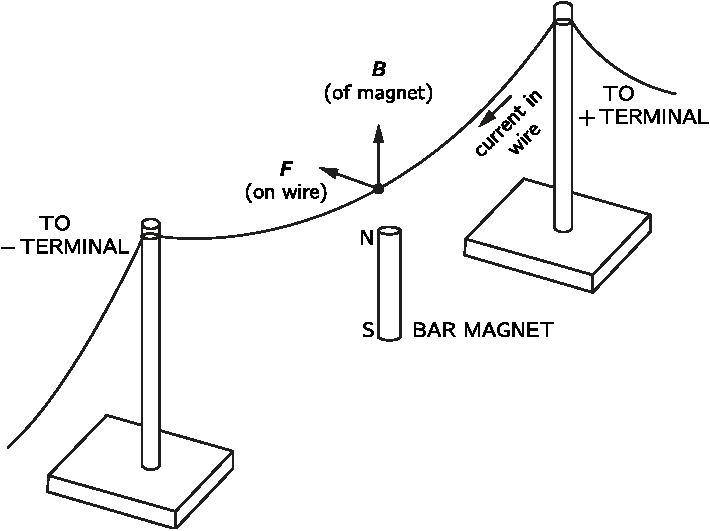
\includegraphics[width=1\linewidth]{fyz_fig148.pdf}
      \caption{Tyčový magnet vyvolává ve vodiči pole \(\vec{B}\). Když vodičem prochází proud,     
               působením síly \(\vec{F} = q\vec{v}\times\vec{B}\) se vodič pohne.
               \cite[s.~20]{Feynman02}}
      \label{fyz:fig148}
    \end{figure}
    
    Účinkem síly \(\vec{F} = q\vec{v}\times\vec{B}\) se při zapnutí proudu vodič pohne. Po dobu 
    trvání proudu se náboje uvnitř vodiče pohybují, tj. mají rychlost \(\vec{v}\), a proto na ně 
    působí magnetické pole magnetu, což se projeví pohybem vodiče do strany.
    
    Když se vodič pohne doleva, je třeba čekat, že magnet dostane náraz směrem doprava. (V opačném 
    případě bychom mohli celé zařízení umístit na vůz a měli bychom pohonný systém, který 
    nezachovává hybnost!) I když je síla příliš malá na to, aby byl pohyb tyčového magnetu 
    viditelný, jemněji uložený magnet, např. střelka kompasu, by se pohnul.
    
    Jak působí na magnet vodič elektrického proudu? Proud ve vodiči vytváří vlastní magnetické 
    pole, které se projeví silovým působením na magnet. Podle posledního členu v rovnici 
    (\ref{FYZ:eq_fey_elmag09}) vyvolá proud nevyhnutelně \emph{cirkulaci pole} \(\vec{B}\) — v 
    tomto případě křivky pole \(\vec{B}\) (magnetické indukční čáry) jsou uzavřené a obepínají 
    vodič, jak je vidět na obr. \ref{fyz:fig149}. Právě toto pole \(\vec{B}\) je původcem 
    síly působící na magnet.  
    
    Podle rovnice (\ref{FYZ:eq_fey_elmag09}) je při stálém proudu cirkulace pole \(\vec{B}\) stejná 
    pro jakoukoliv křivku, která vodič obepíná. Křivky, např. kružnice, které jsou dále od vodiče, 
    mají obvod větší, takže tangenciální složka \(\vec{B}\) musí být menší. Vidíte, že podle 
    očekávání bude pole \(\vec{B}\) klesat nepřímo úměrně vzdálenosti od dlouhého přímého 
    vodiče.     

    \begin{figure}[ht!]
      \centering
      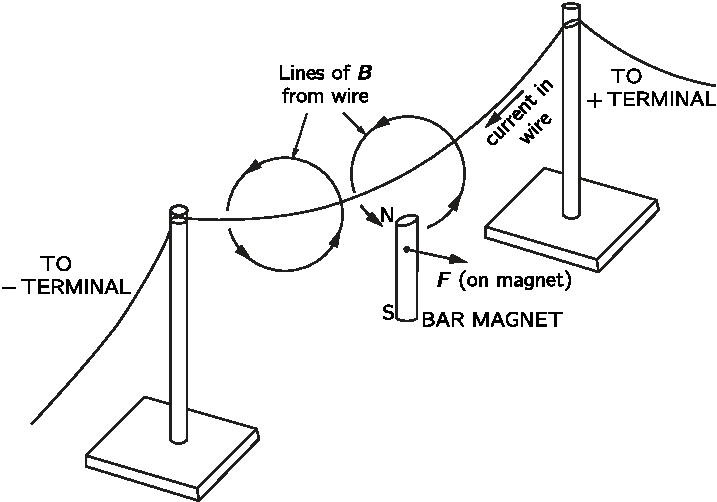
\includegraphics[width=1\linewidth]{fyz_fig149.pdf}
      \caption{Magnetické pole vodiče působí silou na magnet.
              \cite[s.~21]{Feynman02}}
      \label{fyz:fig149}
    \end{figure}
    
    Řekli jsme, že proud ve vodiči vytváří magnetické pole a že v magnetickém poli působí na vodič, 
    kterým prochází proud, síla. Pak bychom měli také očekávat, že vytvoříme-li magnetické pole 
    proudem v jednom vodiči, bude působit silou na jiný vodič, kterým také prochází proud. Můžeme 
    si to ukázat na dvou visících vodičích, jako na obr. \ref{fyz:fig150}. Mají-li proudy 
    stejný směr, vodiče se přitahují, jsou-li proudy opačného směru, vodiče se odpuzují.
    
    Krátce řečeno elektrické proudy vytvářejí magnetická pole právě tak jako magnety. Ale počkejte, 
    co je vlastně magnet? Jestliže pohybující se náboje vyvolávají magnetická pole, není možné, že 
    magnetické pole kousku železa je ve skutečnosti také důsledkem proudů? Ukazuje se, že ano. 
    Tyčový magnet z našeho pokusu můžeme nahradit cívkou navinutou z drátu, stejně jako na obr. 
    \ref{fyz:fig151}. Prochází-li cívkou proud (jakož i přímým vodičem nad ní), pozorujeme 
    pohyb vodiče přesně jako předtím, kdy jsme měli místo cívky magnet. Jinak řečeno, proud v cívce 
    imituje magnet. Ukazuje se tedy, že kus železa působí tak, jako kdyby obsahoval ustavičně 
    obíhající proud. Magnety opravdu můžeme objasnit pomocí permanentních proudů v atomech železa. 
    Sílu účinkující na magnet na obr. \ref{fyz:fig149} vyvolává tedy druhý člen ve vztahu 
    (\ref{FYZ:eq_fey_elmag01})         

    \begin{figure}[ht!]
      \centering
      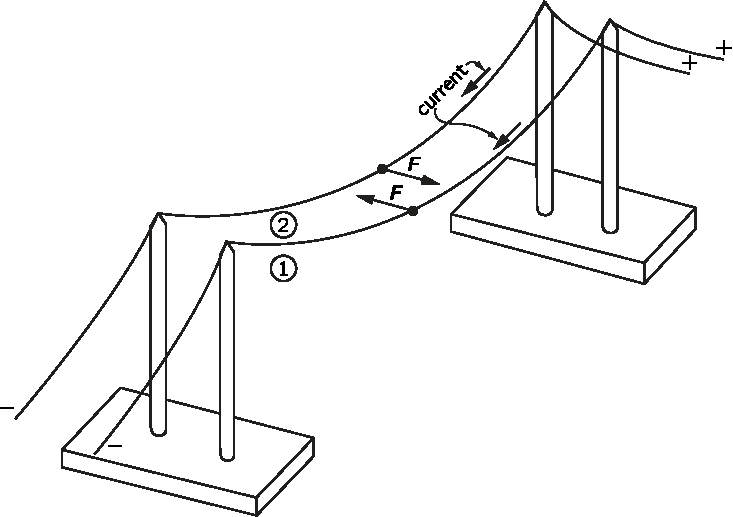
\includegraphics[width=1\linewidth]{fyz_fig150.pdf}
      \caption{Dva vodiče, kterými prochází proud, na sebe navzájem působí silami.
               \cite[s.~21]{Feynman02}}
      \label{fyz:fig150}
    \end{figure}
    
    Odkud se tyto proudy berou? Jednou z možností je, že z pohybu elektronů v atomových orbitách. 
    To však není případ železa, třebaže to tak v některých látkách je. Kromě oběhu v atomu se 
    elektron otáčí i kolem své vlastní osy (nějak podobně jako vlastní rotace Země) a právě tento 
    pohyb, tzv. spin elektronu, vytváří magnetické pole v případě železa. (Říkáme, že je to „něco 
    podobného“ jako vlastní rotace Země, protože tento problém zasahuje tak hluboko do kvantové 
    mechaniky, že klasické představy opravdu příliš dobře nevystihují tyto poměry.) Ve většině 
    látek se některé elektrony otáčejí jedním směrem, kdežto jiné směrem opačným, takže jejich 
    magnetizmus se vyruší. Ale v železe - ze záhadného důvodu, o němž budeme hovořit později - jsou 
    osy otáčení mnoha elektronů uspořádány jedním směrem, a to je zdrojem magnetizmu.
    
    Protože pole magnetů pocházejí z proudů, nemusíme do rovnic (\ref{FYZ:eq_fey_elmag08}) nebo
    (\ref{FYZ:eq_fey_elmag09}) přidávat žádný zvláštní člen zohledňující magnety. Stačí zahrnout 
    všechny proudy včetně těch, které souvisejí se spiny elektronů, a zákon bude správně. Také 
    byste si měli všimnout, že podle rovnice (\ref{FYZ:eq_fey_elmag09}) neexistují magnetické 
    „náboje“ analogické s elektrickými, vystupující na pravé straně rovnice 
    (\ref{FYZ:eq_fey_elmag07}). Žádné se nenašly.

    \begin{figure}[ht!]
      \centering
      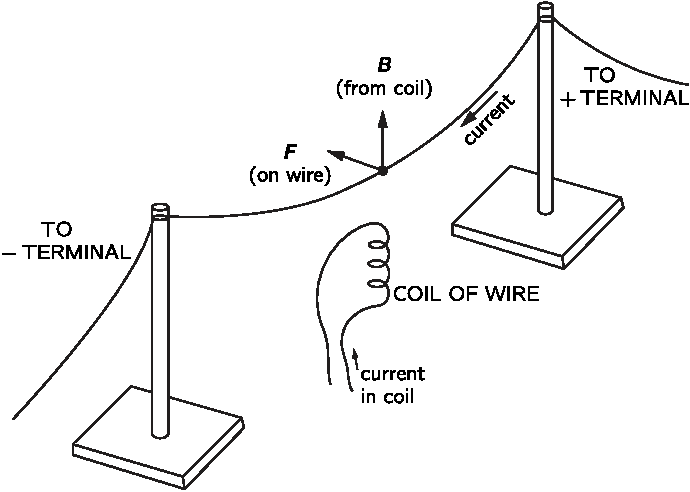
\includegraphics[width=1\linewidth]{fyz_fig151.pdf}
      \caption{Tyčový magnet na obr. \ref{fyz:fig148} je možné nahradit cívkou s      
               elektrickým proudem. Na vodič přitom působí podobná sila.
              \cite[s.~22]{Feynman02}}
      \label{fyz:fig151}
    \end{figure} 

    První člen na pravé straně rovnice (\ref{FYZ:eq_fey_elmag09}) objevil Maxwell čistě teoreticky 
    a je velmi důležitý. Podle něj mají proměnlivá elektrická pole magnetické účinky. Pravda je, že 
    bez tohoto členu by rovnice neměla smysl, protože bez něho by neexistovaly elektrické proudy v 
    obvodech, které netvoří uzavřené smyčky. Ale, jak uvidíme na následujícím příkladě, takové 
    proudy existují. Představme si kondenzátor skládající se ze dvou rovinných desek. Nechť se 
    nabíjí proudem směřujícím k jedné desce a vycházejícím z druhé z nich (obr. 
    \ref{fyz:fig040}). Opišme okolo jednoho z přívodů křivku \(C\), jejíž vnitřek vyplníme 
    plochou \(S_1\), která přetíná vodič (viz obrázek). Podle (\ref{FYZ:eq_fey_elmag09}) je 
    cirkulace \(\vec{B}\) podél \(C\) určena proudem ve vodiči. Ale co když vnitřek křivky \(C\) 
    vyplníme jinou plochou \(S_2\), která má tvar mísy a prochází mezi deskami kondenzátoru, 
    přičemž se nikde nedotýká vodiče. Touto plochou jistě neprochází žádný proud. A zajisté 
    změna umístění myšlené plochy nezmění reálné magnetické pole! Cirkulace pole \(\vec{B}\) se 
    tedy nesmí změnit. První člen na pravé straně rovnice (\ref{FYZ:eq_fey_elmag09}) se ve 
    skutečnosti kombinuje s druhým členem tak, aby složením daly shodné výsledky pro obě plochy 
    \(S_1\) a \(S_2\). V případě \(S_2\) se cirkulace \(\vec{B}\) udává pomocí rychlosti změny toku 
    pole \(\vec{E}\) mezi deskami kondenzátoru. Vychází, že změna \(\vec{E}\) je právě v takovém 
    poměru k proudu, aby rovnice (\ref{FYZ:eq_fey_elmag09}) byla správná. Maxwell viděl tuto 
    potřebu a byl prvním, kdo napsal úplnou rovnici.

    \begin{figure}[ht!]  %\ref{fyz:fig040}
      \centering
      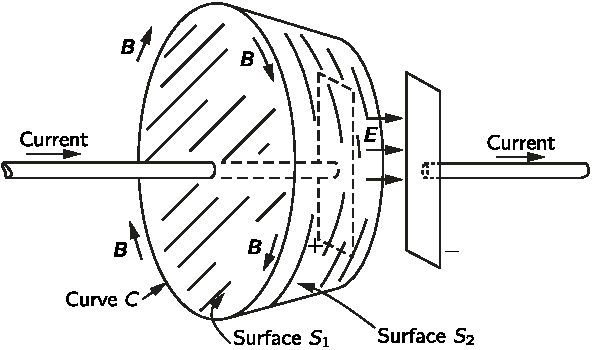
\includegraphics[width=0.7\linewidth]{fyz_fig040.pdf}
      \caption{Cirkulace vektoru \(\vec{B}\) po křivce \(C\) je určena buď proudem procházejícím 
               plochou \(S_1\) nebo rychlosti změny toku vektoru \(\vec{E}\) plochou \(S_2\).
               \cite[s.~23]{Feynman02}}
      \label{fyz:fig040}
    \end{figure}      
    Zařízením znázorněným na obr. \ref{fyz:fig040} můžeme demonstrovat další ze zákonů   
    elektromagnetizmu. Odpojme konce zavěšeného vodiče od akumulátoru a připojme je ke 
    galvanometru, který nám ukazuje, jestli vodičem protéká proud. Když vodič postrčíme do strany v 
    magnetickém poli magnetu, zaznamenáme proud. Takový jev je opět dalším důsledkem vztahu 
    (\ref{FYZ:eq_fey_elmag01}) — na elektrony ve vodiči působí síla \(\vec{F}=q\vec{v} 
    \times\vec{B}\). Elektrony mají příčnou rychlost, neboť se pohybují s vodičem. Rychlost \(v\) v 
    kombinaci se svislým \(\vec{B}\) magnetu vyvolává sílu působící na elektrony v podélném směru 
    (vzhledem k vodiči) a uvádí je do pohybu ke galvanometru.      

    Předpokládejme však, že vodič necháme v klidu a pohybujeme magnetem. Na základě principu 
    relativity se domníváme, že by v tom neměl být žádný rozdíl. A opravdu, na galvanometru 
    pozorujeme podobný proud. Jak působí magnetické pole na náboje, které se nepohybují? Podle 
    vztahu (\ref{FYZ:eq_fey_elmag01}) tam musí být elektrické pole. Pohybující se magnet musí 
    vytvořit elektrické pole. Jak k tomu dojde, popisuje kvantitativně rovnice 
    (\ref{FYZ:eq_fey_elmag07}). Tato rovnice popisuje mnoho prakticky důležitých úkazů, např. ty, 
    které se vyskytují v elektrických generátorech a transformátorech.
    
    Nejpozoruhodnějším důsledkem našich rovnic je, že spojením rovnic (\ref{FYZ:eq_fey_elmag07}) a
    (\ref{FYZ:eq_fey_elmag09}) lze vysvětlit vyzařování elektromagnetických vzruchů na velké 
    vzdálenosti. Příčina spočívá zhruba v tomto. Předpokládejme, že někde máme vzrůstající 
    magnetické pole, třeba proto, že jsme např. najednou zapnuli proud ve vodiči. Potom se podle 
    rovnice (\ref{FYZ:eq_fey_elmag07}) musí objevit cirkulace elektrického pole. Když elektrické 
    pole postupně vzrůstá a vytváří svou cirkulaci, bude se podle rovnice 
    (\ref{FYZ:eq_fey_elmag09}) generovat magnetická cirkulace. Ale nárůst tohoto magnetického pole 
    způsobí vznik nové cirkulace elektrického pole atd. Takto si pole razí svou cestu prostorem, 
    aniž by potřebovala náboje nebo proudy někde jinde než ve svém zdroji. Tím způsobem jeden 
    druhého vidíme! To všechno obsahují rovnice elektromagnetických polí.
       
   
  %-------------------- Co jsou pole? --------------------------------------------------------------
  \section{Co jsou pole?}  
    Nyní uděláme několik poznámek o našem způsobu náhledu na tuto otázku. Mohli byste namítnout: 
    „Celá ta záležitost s toky a cirkulacemi je velmi abstraktní. V každém bodu prostoru existují 
    elektrická pole, kromě toho platí určité zákony. Ale co se opravdu děje? Proč to nemůžeme 
    vysvětlit např. tím, ať už je to cokoliv, co prochází mezi náboji?“ Problém je ve našich 
    předsudcích. Mnozí fyzici říkají, že přímé působení bez ničeho mezi působícími objekty je 
    nemyslitelné. Říkají: „Podívejte se, jediné síly, které známe, jsou přímým působením jednoho 
    kousku látky na jiný. Je nemožné, aby existovala síla, jejíž přenos nic nezprostředkuje.“ Ale 
    co se ve skutečnosti děje, když zkoumáme „přímé působení“ jednoho kusu látky na druhý? 
    Zjistíme, že nejde o bezprostřední dotyk obou kusů, kusy jsou od sebe trochu vzdálené a 
    uplatňují se mezi nimi elektrické síly, působící v malém měřítku. Tak docházíme k tomu, že 
    působení ve formě přímého dotyku máme vysvětlovat pomocí elektrických sil. Zajisté by nebylo 
    rozumné trvat na tom, že elektrická síla má vypadat jako staré známé odtlačování nebo 
    přitahování pomocí svalů, zejména když se ukazuje, že svalové účinky je třeba vykládat jako 
    elektrické síly! Jediná otázka, která má smysl, je, jaký způsob popisu elektrických sil je 
    nejvhodnější. Někteří lidé si je vykládají jako působení nábojů na dálku a používají přitom 
    složitý zákon. Jiní si oblíbili siločáry. Celou dobu kreslí siločáry a psát vektory \(\vec{E}\) 
    a \(\vec{B}\) je podle nich příliš abstraktní. Siločáry jsou však jen hrubým způsobem popisu 
    pole a je velmi těžké podat správné kvantitativní zákony bezprostředně pomocí siločar. Kromě 
    toho pojem siločar neobsahuje nejhlubší princip elektrodynamiky - \emph{princip superpozice}, I 
    když víme, jak vypadají siločáry pro jednu množinu nábojů a jak vypadají pro jinou množinu 
    nábojů, neuděláme si z toho žádnou představu o obraze siločar v případě, že množiny působí 
    najednou. Naproti tomu z matematického hlediska je superpozice jednoduchá - prostě sečteme dva 
    vektory. Určitou předností siločar je, že poskytují názorný obraz, ale mají také nevýhody. 
    Způsob uvažování pomocí přímé interakce má velké výhody, když se uvažuje o elektrických 
    nábojích v klidu, ale má také velké nevýhody, jde-li o náboje v rychlém pohybu.
    
    Nejlepším způsobem je používat abstraktní pojem pole. To, že je abstraktní, je nepříjemné, ale  
    nevyhnutelné. Pokusy popisovat elektrické pole jako pohyb nějakých ozubených koleček, pomocí 
    siločar nebo napětí v nějaké látce si vyžádaly větší úsilí fyziků, než by stačilo na samotné 
    nalezení správných odpovědí na problémy elektrodynamiky. Je zajímavé, že, správné rovnice o 
    chování světla v krystalech vypracoval McCullough už r. 1843. Lidé mu však říkali: „Dobře, ale 
    taková reálná látka, jejíž mechanické vlastnosti by mohly vyhovovat těmto rovnicím, neexistuje, 
    a protože světlo je vlnění, které musí kmitat v něčem, nemůžeme těmto abstraktním rovnicím 
    věřit.“ Kdyby lidé byli bývali méně zaujatí, mohli by uvěřit správným rovnicím chování světla o 
    mnoho dříve.
    
    Co se týče magnetického pole, můžeme udělat následující poznámku: Předpokládejme, že jsme 
    nakonec úspěšně vytvořili obraz magnetického pole pomocí nějakého druhu siločar nebo koleček 
    rychle se otáčejících v prostoru. Pokusme se potom vysvětlit, co se stane se dvěma náboji 
    pohybujícími se v prostoru rovnoběžně stejnou rychlostí. Protože se pohybuji budou se chovat 
    jako dva proudy a každý z nich bude mít svoje magnetické pole (podobně jako proudy ve vodičích 
    na obr. \ref{fyz:fig150}). Pozorovatel, který by se pohyboval spolu s náboji, by je 
    však vnímal jako stojící a tvrdil by, že magnetické pole není. Ozubená kolečka anebo siločáry 
    tedy zmizí, když se pohybujete spolu s objektem! Jediné co jsme udělali je, že jsme vytvořili 
    nový problém. Jak mohou ozubená kola zmizet? Lidé, kteří kreslí siločáry, se dostávají do 
    podobných těžkostí. Nejen, že není možné říci, zda se siločáry s náboji pohybují anebo ne, ale 
    můžou v určitých souřadnicových soustavách zcela zmizet.
    
    To, co bychom ještě chtěli říct, je, že magnetizmus je skutečně relativistickým efektem. V právě
    uvažovaném případě dvou rovnoběžně se pohybujících nábojů lze očekávat, že bude třeba udělat  
    relativistické korekce k jejich pohybu pomocí členů řádu \(\frac{v^2}{c^2}\). Tyto korekce musí 
    odpovídat magnetické síle. Ale co se silou mezi dvěma vodiči v našem pokusu (obr. 
    \ref{fyz:fig150})? Tam je magnetická síla jedinou působící silou. Nevypadá jako 
    „relativistická korekce“. Kromě toho, odhadneme-li rychlosti elektronů ve vodiči (to můžete 
    udělat sami), zjistíme, že jejich střední rychlost podél vodiče je asi 
    \SI{0,01}{\centi\metre\per\second}. Takže \(\frac{v^2}{c^2}\) je asi \(10^{-25}\). Určitě 
    zanedbatelná „korekce“. Ale není! Ačkoli magnetická síla je v tomto případě \(10^{-25}\) 
    „normální“ elektrické síly mezi pohybujícími se elektrony, vzpomeňme si, že „normální“ 
    elektrické síly vymizely v důsledku téměř dokonalého vyrovnání - neboť vodiče mají stejný počet 
    protonů i elektronů. Rovnováha je mnohem přesnější než \(1/10^{-25}\) a malý relativistický 
    člen, který nazýváme magnetickou silou, je jediným členem, který zůstal, a stává se tak 
    dominantním.
    
    Právě téměř dokonalé vzájemné vyrušení elektrických sil umožnilo zkoumat relativistické efekty, 
    tj. magnetizmus, a objevit správné rovnice s přesností \(\frac{v^2}{c^2}\), i když fyzici 
    nevěděli, co se ve skutečnosti děje. A právě proto, když byla objevena teorie relativity, 
    elektromagnetické zákony se nemusely měnit. Na rozdíl od mechaniky už byly správné s přesností 
    \(\frac{v^2}{c^2}\).
    
    Elektromagnetické pole je rozloženo v prostoru a může se měnit s časem. Veličiny, které toto
    pole popisují jsou obecně funkcí času a tří geometrických souřadnic. Podle časového průběhu
    rozlišujeme:
    \begin{enumerate}
      \item \emph{pole časově neproměnné}: jsou-li náboje v klidu, budeme hovořit o poli
            \emph{statickém}, jsou-li v rovnoměrném pohybu (tj. tvoří-li stejnosměrný proud),
           jde o pole \emph{stacionární}.
      \item \emph{pole časově proměnně} čili \emph{nestacionární}: jestliže se
            elektromagnetické pole mění s časem relativně pomalu, nazýváme jej
            \emph{kvazistacionárním}. Jestliže se mění s časem periodicky, říkáme, že je v
            \emph{ustáleném stavu}. Speciální případy jsou:
            \begin{itemize}
              \item \emph{harmonický ustálený stav}: pole se časem mění podle sinové nebo
                    kosinové funkce
               \item \emph{neustálený (přechodný) stav}: pole přechází z jednoho ustáleného
                     stavu do druhého. Tento případ nastane tehdy, když zdroje pole změní své
                     parametry, resp. svou polohu v prostoru.
            \end{itemize}
    \end{enumerate}
  
    Podle prostorového průběhu rozlišujeme:
    \begin{enumerate}
      \item \emph{trojrozměrné}: (trojdimenzionální, prostorové pole), veličiny
            charakterizující pole jsou funkcemi tří geometrických souřadnic ( např. $x, y, z$).
            Označení: \emph{3D pole}.
      \item \emph{dvojrozměrné}: (dvojdimenzionální pole), veličiny charakterizující pole jsou
            funkcemi dvou  geometrických souřadnic. Dvourozměrné pole je např. pole rovinné (je
            funkcí souřadnic x, y), nebo pole rotačně souměrné (je funkcí r, z). Označení: 2D
            pole.
      \item \emph{jednorozměrné}: (jednodimenzionální pole), veličny charakterizující pole jsou
            funkcemi jedné geometrické souřadnice (např. x, nebo r). Označení: 1D.
      \item \emph{homogenní}: veličiny charakterizující pole jsou v kterémkoliv bodě uvažované
            oblasti prostoru tytéž. (tj. jsou nezávislé na geometrických souřadnicích).
    \end{enumerate}      
    \begin{figure}[ht!]
      \centering
      \begin{tabular}{cc}
       \subfloat[3D úloha: jiskřiště hrot - deska ]{\label{fyz:fig221a}
         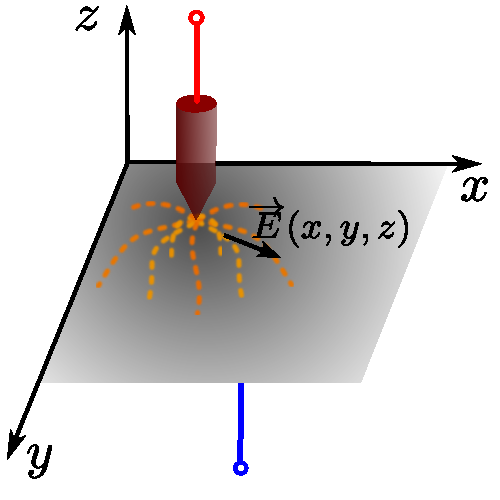
\includegraphics[width=0.4\linewidth]{fyz_fig221a.pdf}}                      &
       \subfloat[2D úloha: dvouvodičové vedení]{\label{fyz:fig221b}
         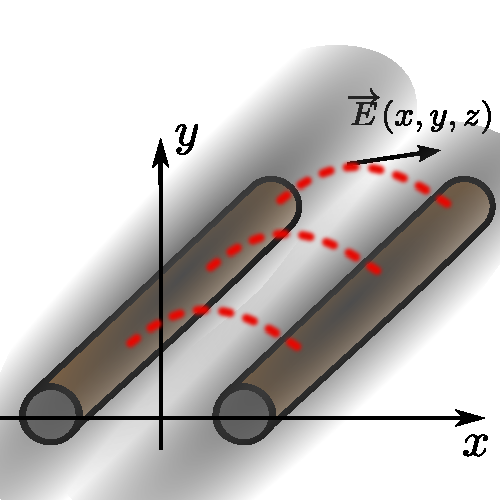
\includegraphics[width=0.4\linewidth]{fyz_fig221b.pdf}}                      \\
       \subfloat[1D úloha: koaxiální kabel]{\label{fyz:fig221c}
         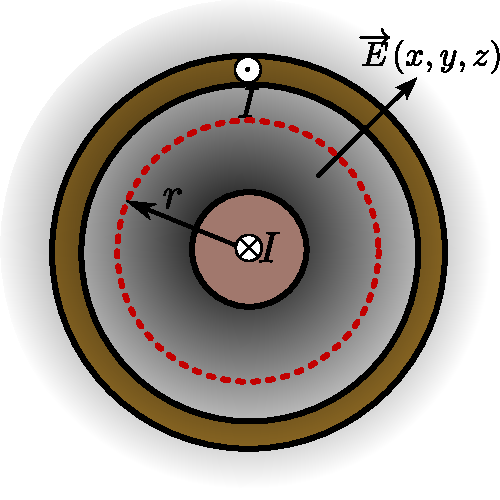
\includegraphics[width=0.4\linewidth]{fyz_fig221c.pdf}}                      &
       \subfloat[1D úloha: deskový kondezátor]{\label{fyz:fig221d}
         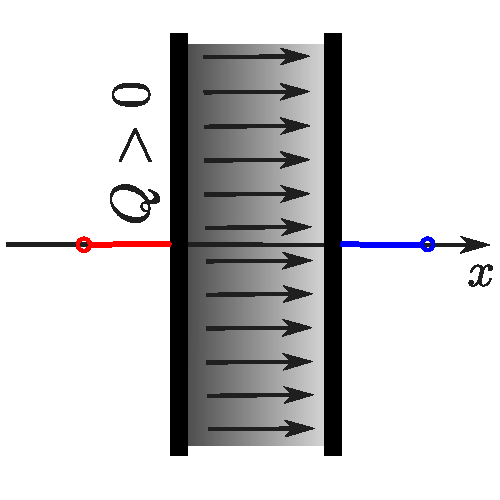
\includegraphics[width=0.4\linewidth]{fyz_fig221d.pdf}}  
      \end{tabular}                          
      \caption{Příklad trojdimenzionálního a), dvojdimenzionálního b) a jednodimenzionálního c), 
               d) pole}
      \label{fyz:fig221}
    \end{figure} 
         
  %------------ Působení na dálku versus teorie pole -----------------------------------------------
  \section{Působení na dálku versus teorie pole}
    Klasická teorie elektromagnetického pole se vynořila ve více méně kompletní formě v roce 1873 v 
    práci \emph{Jamese Clerka Maxwella} „Pojednání o elektřině a magnetismu“. Maxwell založil svojí 
    teorii z větší části na intuitivních úvahách \emph{Michaela Faradaye}. Široké přijetí 
    Maxwellovy teorie způsobilo zásadní posun našeho poznání fyzikální reality. V této teorii jsou 
    elektromagnetická pole zprostředkovateli interakce mezi hmotnými objekty. Tento pohled se 
    radikálně liší od staršího pohledu „působení na dálku“, který předcházel teorii pole.
  
    Co je „působení na dálku“? Je to pohled na svět, ve kterém interakce dvou hmotných objektů 
    nevyžaduje žádný jiný mechanismus než objekty samotné a prázdný prostor mezi nimi. To znamená, 
    že objekty na sebe navzájem působí silou jednoduše díky svojí přítomnosti. Jakékoliv vzájemné 
    síly mezi nimi (na příklad gravitační nebo elektromagnetické) jsou okamžitě přenášeny z jednoho 
    objektu na jiný skrze prázdný prostor. Není zde potřeba zahrnout jinou metodu nebo 
    zprostředkovatele takovýchto sil, či konečnou rychlost šíření zprostředkovaného přenosu. To je 
    známo jako „silové působení na dálku“, protože kromě objektů působících na sebe „silou“ a 
    „vzdálenosti“ mezi nimi není již v prázdném prostoru zahrnuto nic. Žádný jiný mechanismus nebo 
    zprostředkovatel není potřeba.
  
    Mnoho vědců mělo námitky proti modelu „působení na dálku“, protože odporoval jejich každodenním 
    zkušenostem, že silou může působit objekt na jiný jen v případě, když jsou v přímém kontaktu. V 
    teorii pole je tento pohled pravdivý jen v určitém smyslu. To znamená, že objekty, které nejsou 
    v přímém kontaktu (objekty oddělené zjevně prázdným prostorem) musí na sebe navzájem silově 
    působit \emph{prostřednictvím jakéhosi média nebo mechanismu nalézajícím se v prostoru mezi 
    objekty}.
  
    Síla mezi dvěma objekty je přenášena přímým „kontaktem“ prvního tělesa na zprostředkující 
    mechanismus (médium) bezprostředně obklopující tento objekt. Poté ji tento prvek prostoru předá 
    sousednímu, ten dalšímu a tímto plynulým způsobem je síla přenesena na médium bezprostředně 
    obklopující druhý objekt a z toho nakonec na objekt samotný.
  
    Ačkoliv dva objekty nejsou v přímém kontaktu společně navzájem, jsou v přímém kontaktu s médiem 
    nebo mechanismem, které existují mezi nimi. Síla mezi objekty je přenášena (konečnou rychlostí) 
    jakýmsi tlakem vyvolaným prostorem ležícím mezi nimi. Pohled „teorie pole“ se tak vyhýbá pojmu 
    „působení na dálku“ a nahrazuje jej pojmem „působení nepřetržitým kontaktem“. Tento „kontakt“ 
    je způsobený tlakem nebo „polem“ indukovaným v prostoru mezi objekty pouhou jejich přítomností.

    Tato myšlenka je podstatou teorie pole a je také základem všech moderních teorií popisujících 
    svět okolo nás. Klasická teorie elektřiny a magnetizmu byla první teorií pole. Na závěr uveďme 
    definici pojmu „pole”, vystihující předchozí ideje
    \begin{definition}
      \textbf{Fyzikální pole} jsou vesměs zprostředkovateli vzájemného působení (interakcí) mezi 
      hmotnými objekty. Např. \emph{elektromagnetické pole je specifická forma hmoty}. Základní 
      vlastnosti má společné s ostatními formami hmoty: je objektivní realitou existující nezávisle 
      na našem vědomí, přísluší mu určitá energie, hmotnost a hybnost, přičemž pro tyto veličiny 
      platí zákony zachování, má kvantovou strukturu (elementární částice elektromagnetického pole 
      se nazývají fotony) a stejně jako ostatní elementární částice mohou projevovat též vlnový 
      charakter. Elektromagnetické pole je zprostředkovatelem elektromagnetických interakcí v 
      makroskopickém i mikroskopickém měřítku a přitom však může existovat i mimo látkové objekty 
      samostatně ve formě elektromagnetického vlnění.
    \end{definition}                 

  %----------------------- Elektromagnetizmus ve vědě a technice -----------------------------------
  \section{Elektromagnetizmus ve vědě a technice}  
    \cite[s.~25]{Feynman02} Tuto kapitolu zakončíme poukázáním na to, že mezi mnohými jevy, které 
    zkoumali Řekové, byly dva velmi neobvyklé. Když třete kousek jantaru, můžete jím zvednout malé 
    kousky papyru. Dále to byl podivný kámen z okolí města Magnesia v Malé Asii, který přitahoval 
    železo. Je těžké si představit, že toto byly jediné dva Řekům známé úkazy, v nichž se projevují 
    elektrické a magnetické účinky. Důvod, že  to opravdu byly jediné dva úkazy, které byly tehdy 
    známy, spočívá především ve fantastické přesnosti vyrovnání nábojů, o níž jsme se zmínili 
    dříve. Práce vědců, kteří přišli po Řecích a kteří objevovali jeden nový jev za druhým, byly 
    vlastně jen různými aspekty těchto vlastností jantaru a magnetovce. Dnes si uvědomujeme, že i 
    jevy chemické interakce a konec konců i samotného života je třeba objasňovat pomocí 
    elektromagnetizmu.

    Současně s tím, jak se vyvíjelo chápání elektromagnetizmu, se objevily také technické možnosti, 
    o nichž se lidem dříve nesnilo. Stalo se možným posílat zprávy telegrafem na velké vzdálenosti, 
    mluvit s člověkem, který je na kilometry vzdálený, bez jakýchkoliv spojů v meziprostoru. 
    Vznikly obrovské energetické soustavy. Velká vodní turbína spojená stovkami kilometrů drátů se 
    vzdáleným elektromotorem udržuje jeho otáčky ve svém rytmu, tisíce a tisíce vodičů se 
    rozvětvují, desítky tisíc motorů na desetitisících místech pohání stroje v průmyslu i 
    domácnostech, to vše se otáčí a funguje díky poznání zákonů elektromagnetizmu.

    Dnes prakticky využíváme i nejjemnější efekty. Elektrické síly, jakkoliv mohutné, mohou být i 
    velmi slabé a můžeme je řídit a mnoha způsoby využívat. Naše přístroje jsou tak citlivé, že to, 
    co člověk dělá, můžeme rozpoznat podle toho, jak ovlivňuje elektrony v tenké kovové tyči 
    vzdálené stovky kilometrů od něj. Jediné co potřebujeme, je použít tyč jako anténu televizního 
    přijímače.

    Z dlouhodobého pohledu historie lidstva, tak, jak se bude jevit, například, za deset tisíc let, 
    lze sotva pochybovat, že Maxwellův objev zákonů elektrodynamiky bude hodnocen jako 
    nejvýznamnější událost 19. století. V porovnání s touto důležitou vědeckou událostí upadne 
    americká občanská válka z téhož desetiletí do provinční bezvýznamnosti.

%} %tikzset
%~~~~~~~~~~~~~~~~~~~~~~~~~~~~~~~~~~~~~~~~~~~~~~~~~~~~~~~~~~~~~~~~~~~~~~~~~~~~~~~~~~~~~~~~~~~~~~~~~~
\printbibliography[title={Seznam literatury}, heading=subbibliography]
\addcontentsline{toc}{section}{Seznam literatury}
